\documentclass[12pt]{article}
\usepackage[utf8]{inputenc}
\usepackage[a4paper, top=2cm, left=3cm, right=3cm, bottom=3cm]{geometry}

\usepackage{graphicx}
\usepackage{authblk}
\usepackage[
    backend = biber,
    style = apa
]{biblatex}
\addbibresource{reference.bib}
\usepackage[skip=20pt]{parskip}
\setlength{\parindent}{20pt}
\usepackage[hidelinks]{hyperref}
\usepackage{url}
\usepackage{caption}
\usepackage{subcaption}


\title{Effects of different levels of nitrogenous and phosphatic fertiliser on plant yield}
\author{Cameron Dixon (49626128)}
\author{Hyeonbin Sirichanchaikul (49601929)}
\affil{The University of Queensland}
\date{\today}


\begin{document}

\maketitle

\section{Introduction}
The presence of Nitrogen (N) and Phosphorous (P) in fertilisers is known to promote the growth of plants as it is essential for the photosynthesis process. 
However, it is possible that when used in combination, N and P could possibly interact in a way that affects the absorption of each nutrient and hence the optimal levels of each in the fertiliser.
By conducting this statistical experiment, we first aim to confirm the relationship between N and P levels in fertiliser with crop yield.
Then, we will test for a relationship between the levels of each chemical with the optimal level of the other.
The null hypothesis ($H_0$) for this experiment will be that there is no relationship between the two variables and the total crop yield.
\begin{itemize}
    \item criteria sheet says to talk about why the study is interesting. i might've messed up by picking plants, sorry about that. good luck
    \item also the introduction should probably have some references. looking at examples, we should probably include something about nitrogenous and phosphatic fertilisers and what we already know about how they affect crop yield.
\end{itemize}


\section{Methods}
\textit{The Islands} are made up of three separate islands, with each containing a "field station".
Each field station is divided into 36 individual plots, where the levels of N and P each plot can be controlled individually of others.
We tested a range of different levels of N and P in the fertilisers (None, Medium, High) for a total of 9 distinct options.
Each option was tested on a sample size of 12 plots and without further intervention, the total crop yield for each plot was measured after 2 days.
While the actual quantity of each level of the chemicals is unknown, it was assumed that the proportions of the quantity between each level is linear in that 'High - Medium' = 'Medium - Low' and 'High $>$ Medium $>$ Low'.

The purpose of this experimental study determine whether
\begin{itemize}
    \item the level of nitrogenous fertiliser affects crop yield
    \item the level of phosphatic fertiliser affects crop yield
    \item an interaction effect between the level of nitrogenous and phosphatic fertiliser affects crop yield
\end{itemize}
The Island consist of 3 islands, with each island having a field station.
Each field station is divided into 36 different plots.
Each p different levels of nitrogenous and phosphatic fertilisers.
2 days after
\subsection{Statistical Model}
The statistical model used for this study will be a two-factor ANOVA model.

\subsection{Hypothesises}
Our null hypothesis \(H_0\) will be

\section{Results}
\begin{figure}[ht]
    \centering
    \caption{Summary of Data}
    \begin{tabular}{c|c|c|c|c}
         \textbf{Nitrogen Level} & \textbf{Phosphate Level} & \textbf{Mean Yield} & \textbf{SD} & \textbf{n}\\ \hline
         None & None & 22.67 & 1.50 & 12\\
         None & Medium & 28.08 & 0.67 & 12\\
         None & High & 31.08 & 1.44 & 12\\
         Medium & None & 25.83 & 2.55 & 12\\
         Medium & Medium & 31.83 & 2.69 & 12\\
         Medium & High & 33.33 & 3.45 & 12\\
         High & None & 30.92 & 3.34 & 12\\
         High & Medium & 36.42 & 2.54 & 12\\
         High & High & 37.83 & 2.72 & 12
    \end{tabular}
\end{figure}
\vspace{3em}
\begin{figure}[ht]
    \centering
    \caption{Two-factor ANOVA table}
    \begin{tabular}{cccccc}
    \hline
    \makecell{Source\\ of Variation} & \makecell{Degrees\\ of Freedom} & \makecell{Sum\\ of Squares} &  \makecell{Mean\\ of Squares} & F value & \(P(f > F)\)\\ \hline
    Nitrogenous & 2 & 1105.56 & 552.78 & 89.7131 & \(<\)2e-16\\
    Phosphatic & 2 & 1123.39 & 561.69 & 91.1602 & \(<\)2e-16\\
    Interaction & 4 & 11.72 & 2.93 & 0.4756 & 0.7535\\
    Error & 99 & 610.00 & 6.16\\ \hline
    \end{tabular}
\end{figure}

\begin{figure}[ht]
    \centering
    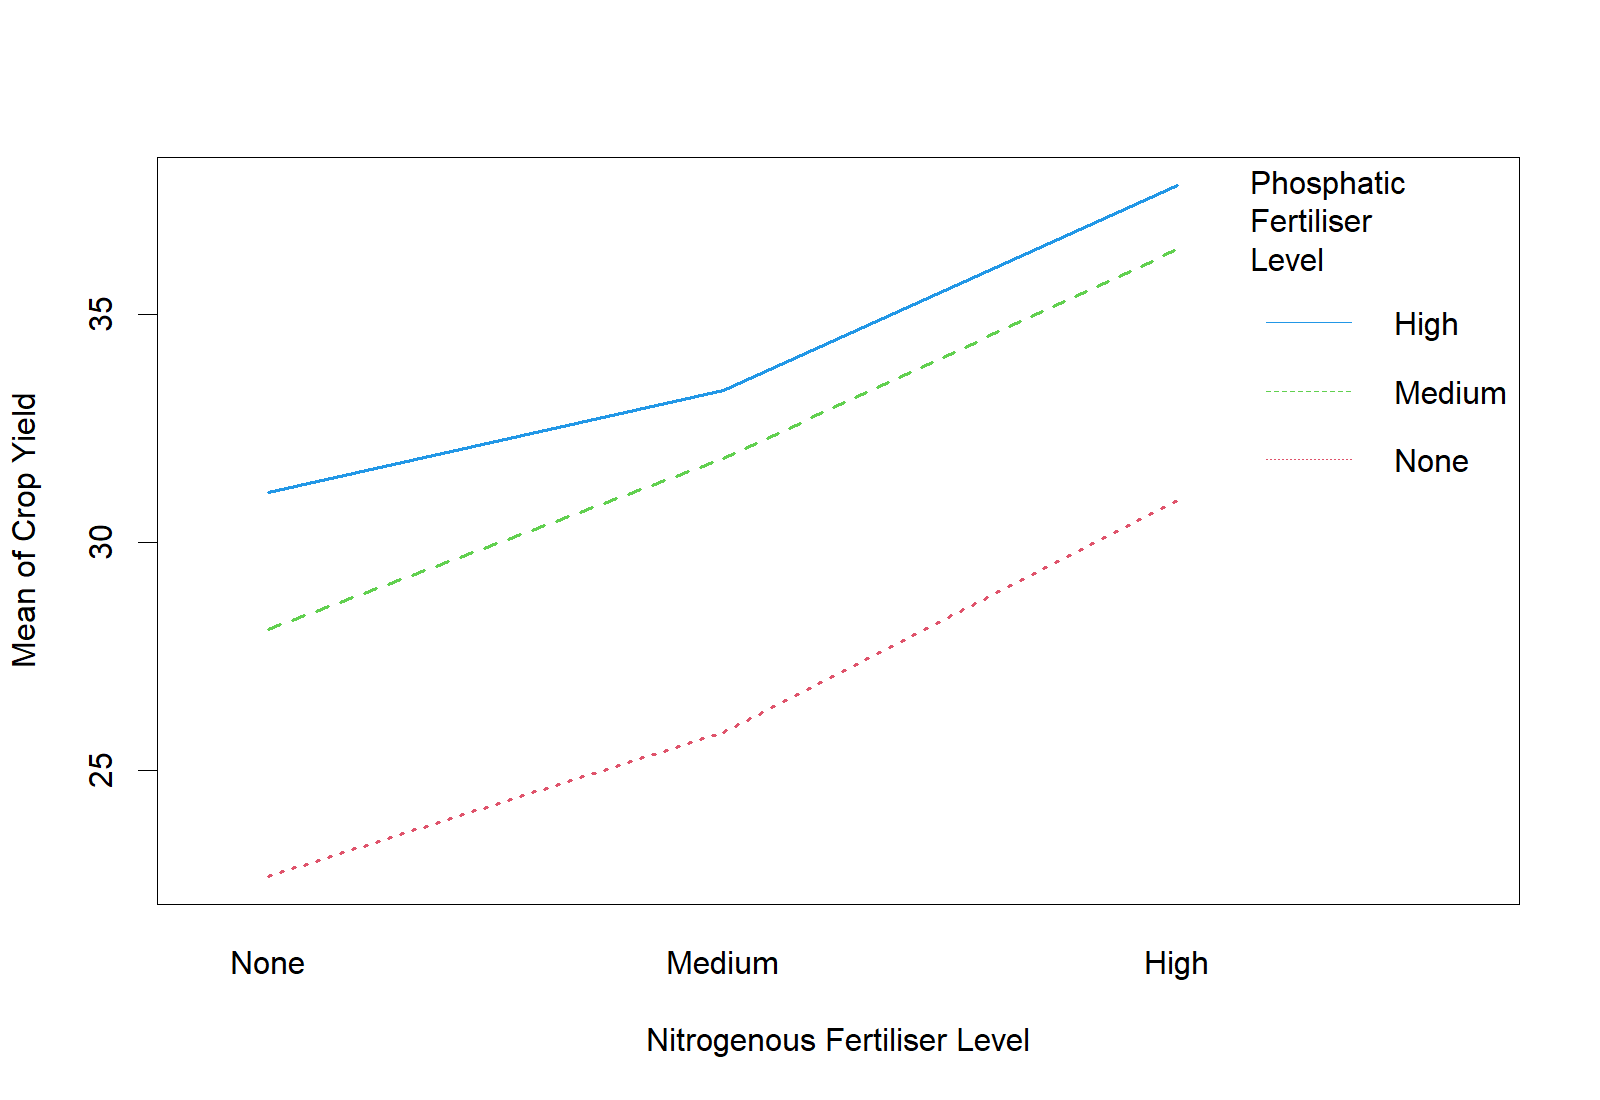
\includegraphics[width=0.8\linewidth]{Figures/Interaction Plot (Nitrogenous).png}
    \caption{Interaction Plot (Nitrogenous)}
\end{figure}

\begin{figure}[ht]
    \centering
    \caption{Interaction Plot (Phosphatic)}
    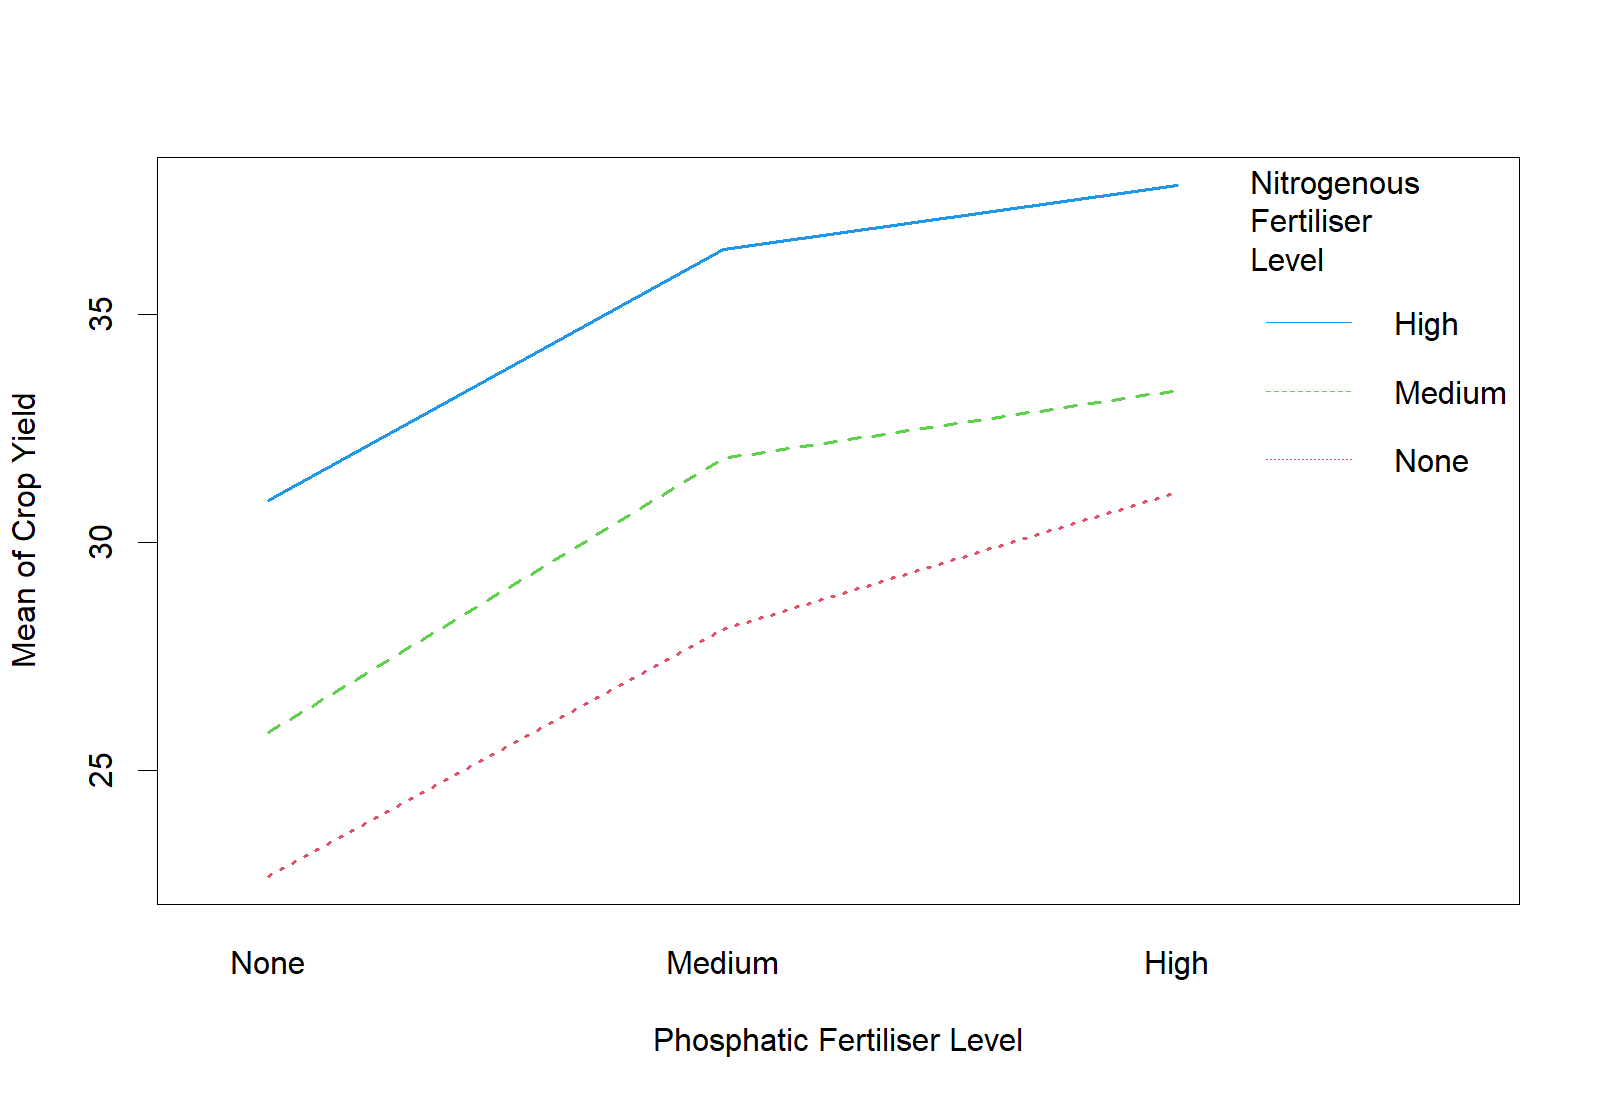
\includegraphics[width=0.8\linewidth]{Figures/Interaction Plot (Phosphatic).png}
\end{figure}


\section{Discussion}
\begin{itemize}
    \item p values are significant for nitrogenous and phosphatic, but not for interaction
    \item should reject null hypothesis for nitrogenous and phosphatic, fail to reject interaction null hypothesis
    \item both interaction plots show little variation in gradient between the different coloured lines, visual evidence of little interaction effect
    \item need limitations: could talk about harvesting plants after 2 days, maybe too short due to time constraints (real reason is didnt know if they would keep growing btw). maybe an interaction couldve occured over long term?
    \item any other limitations
\end{itemize}

\section{Conclusion}
\begin{itemize}
    \item can summarise results if want, this section might not be needed though
\end{itemize}

\newpage

\printbibliography
\end{document}